%\subsection{Modules and skip connections}\label{sec:skip}
\subsection{Modules}\label{sec:skip}

Deep neural nets are essentially composition of many nonlinear functions. A component function may be designed to have specific properties in a given task, and it can be itself resulted from composing a few simpler functions. In LSTM, we have seen that the building block consists of several intermediate variables, including cell states and forget gates that can capture long-term dependency and alleviate numerical issues. 

This leads to the idea of designing \textit{modules} for building more complex neural net models. Desirable modules usually have low computational costs, alleviate numerical issues in training, and lead to good statistical accuracy. Since modules and the resulting neural net models form computational graphs, training follows the same principle briefly described in Section~\ref{sec:super}.

Here, we use the examples of \emph{Inception} and \emph{skip connections} to illustrate the ideas behind modules. 
Figure~\ref{fig:skip}(a) is an example of ``Inception'' modules used in GoogleNet~\citep{szegedy2015going}. As before, all the convolutional layers are followed by the ReLU activation function. The concatenation of information from filters with different sizes give the model great flexibility to capture spatial information. Note that $1 \times 1$ filters is an $1 \times 1 \times d_3$ tensor (where $d_3$ is the number of feature maps), so its convolutional operation does not interact with other spatial coordinates, only serving to aggregate information from different feature maps at the same coordinate. This reduces the number of parameters and speeds up the computation. Similar ideas appear in other work \citep{lin2013network, iandola2016squeezenet}.

%\begin{figure}[H]\label{fig:skip}
%    \centering
%    \begin{subfigure}[b]{0.5\textwidth}
%	\centering
%        \includegraphics[scale = 0.5]{Figure/inception}
%	\caption{The ``Inception'' module from GoogleNet. \texttt{Concat} means combining all features maps into a tensor. }
%    \end{subfigure}
%	~
%    \begin{subfigure}[b]{0.4\textwidth}
%	\centering
%        \includegraphics[scale = 0.5]{Figure/resnet2}
%	\caption{Skip connections are added every two layers in ResNets. }
%    \end{subfigure}
%    %\caption{Pictures of animals}\label{fig:animals}
%\end{figure}

\begin{figure}[htb!]
\centering
\begin{tabular}{cc}
\includegraphics[scale = 0.5]{inception} & \includegraphics[scale = 0.5]{resnet2} \tabularnewline
(a) ``Inception'' module & (b) Skip connections
\end{tabular}
\caption{(a) The ``Inception'' module from GoogleNet. \texttt{Concat} means combining all features maps into a tensor. (b) Skip connections are added every two layers in ResNets. }\label{fig:skip}
\end{figure}



Another module, usually called \textit{skip connections}, is widely used to alleviate numerical issues in very deep neural nets, with additional benefits in optimization efficiency and statistical accuracy. Training very deep neural nets are generally more difficult, but the introduction of skip connections in \emph{residual networks} \citep{he2016deep, he2016identity} has greatly eased the task. 

The high level idea of skip connections is to add an identity map to an existing nonlinear function. Let $\bF(\xx)$ be an arbitrary nonlinear function represented by a (fragment of) neural net, then the idea of skip connections is simply replacing $\bF(\xx)$ with $\xx + \bF(\xx)$. Figure~\ref{fig:skip}(b) shows a well-known structure from residual networks \citep{he2016deep}---for every two layers, an identity map is added:
\begin{equation}\label{eq:mapsto}
\xx \longmapsto \bsigma(\xx + \bF(\xx)) = \bsigma(\xx + \bW' \bsigma(\bW \xx + \bb) + \bb'),
\end{equation}
where $\xx$ can be hidden nodes from any layer and $\bW, \bW', \bb, \bb'$ are corresponding parameters. By repeating (namely composing) this structure throughout all layers, \cite{he2016deep, he2016identity} are able to train neural nets with hundreds of layers easily, which overcomes well-observed training difficulties in deep neural nets. Moreover, deep residual networks also improve statistical accuracy, as the classification error on ImageNet challenge was reduced by $46\%$ from 2014 to 2015. As a side note, skip connections can be used flexibly. %, and they can be combined with other ideas and modules to form complex deep neural nets.
They are not restricted to the form in \eqref{eq:mapsto}, and can be used between any pair of layers $\ell, \ell'$ \citep{Huang17}. 

%\subsection{Note}
%Convolutional neural networks can be traced back to the \emph{Neocognitron} model \citep{fukushima1982neocognitron}, where later it was combined with gradient-based training for classification \citep{lecun1998gradient}. The revolved interest in CNN in this century began with the success of AlexNet, a specific convolutional neural network, in ImageNet Challenge \citep{krizhevsky2012imagenet}. VGGNet \citep{simonyan2014very} greatly simplifies the structure of CNN and made a first step towards deeper CNN (VGGNet has 19 layers, compared with 8 layers in AlexNet). In 2016, He et.~al. \citep{he2016deep} proposed a new convolutional neural network, called \emph{ResNet}, where it adds \emph{skip connections} every two convolutional layers. This ``small'' change of structure enables the training of very deep neural nets (152 layers therein) and achieves state-of-the-art results in several standard image processing tasks. 

